% !TEX root = ../Main.tex
\chapter{空间角、距离与向量}

线、面理顺之后，还要会算空间里的"角"和"距离"。这一章把三类角、几类距离的定义列清楚，再交代空间向量法——后面综合题里求角、求距离基本都靠它。

\section{基本概念补充：三类角}

\state{线线角}{
    两条异面直线所成的角 $\alpha$，$\alpha\in[0^\circ,90^\circ]$。把两条线平移到相交，取所成的锐角（或直角）。
}

\state{线面角}{
    直线 $l$ 与平面 $\alpha$ 所成的角 $\theta$，$\theta\in[0^\circ,90^\circ]$。

    \textbf{找角的方法}：在 $l$ 上取一点 $P$，作 $PO\perp\alpha$（$O$ 为垂足），$A$ 为 $l$ 与 $\alpha$ 的交点，则 $\theta=\angle PAO$（斜线与它在面内射影所成的角）。
}

\begin{center}
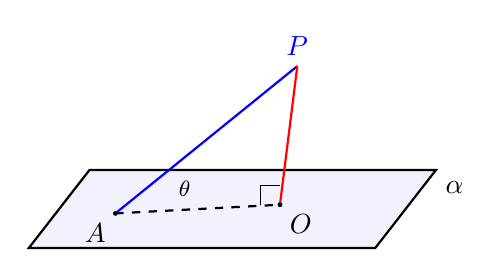
\begin{tikzpicture}[scale=1.1]
    \draw[thick, fill=blue!5] (-2,-0.4) -- (2,-0.4) -- (2.7,0.5) -- (-1.3,0.5) -- cycle;
    \coordinate (A) at (-1,0); \coordinate (O) at (0.9,0.1); \coordinate (P) at (1.1,1.7);
    \draw[thick, blue] (A) -- (P) node[above] {$P$};
    \draw[thick, red] (P) -- (O);
    \draw[thick, dashed] (A) -- (O);
    \draw[thin] (O) ++(-0.22,0) -- ++(0,0.22) -- ++(0.22,0);
    \fill (A) circle (0.8pt) node[below left] {$A$};
    \fill (O) circle (0.8pt) node[below right] {$O$};
    \node at (-0.2,0.08) [above] {\footnotesize $\theta$};
    \node at (2.7,0.3) [right] {$\alpha$};
\end{tikzpicture}
\end{center}

\state{面面角（二面角，即两平面的夹角）}{
    二面角 $\beta$，$\beta\in[0^\circ,180^\circ]$。

    \textbf{找角的方法}：在棱 $l$ 上取一点 $O$，在两个半平面内分别作 $OA\perp l$、$OB\perp l$，则 $\beta=\angle AOB$。
}

\begin{center}
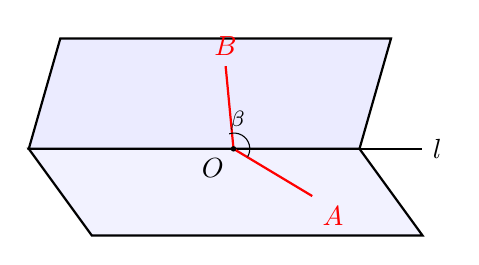
\begin{tikzpicture}[scale=1]
    % 棱 l 沿水平
    \draw[thick] (-2.6,0) -- (2.4,0) node[right] {$l$};
    % 一个半平面（水平）
    \draw[thick, fill=blue!5] (-2.6,0) -- (1.6,0) -- (2.4,-1.1) -- (-1.8,-1.1) -- cycle;
    % 另一个半平面（向上斜）
    \draw[thick, fill=blue!8] (-2.6,0) -- (1.6,0) -- (2.0,1.4) -- (-2.2,1.4) -- cycle;
    \coordinate (O) at (0,0);
    \coordinate (A) at (1.0,-0.6);
    \coordinate (B) at (-0.1,1.05);
    \draw[thick, red] (O) -- (A) node[below right] {$A$};
    \draw[thick, red] (O) -- (B) node[above] {$B$};
    \draw[thin] (O) ++(0.18,-0.1) arc (-30:108:0.2);
    \node at (0.05,0.35) {\footnotesize $\beta$};
    \fill (O) circle (1pt) node[below left] {$O$};
\end{tikzpicture}
\end{center}

\section{几类距离}

\state{常用的距离}{
    \begin{itemize}
        \item 平行平面间的距离；
        \item 异面直线间的距离。
    \end{itemize}
}

\section{空间向量}

立体几何里许多"找角、找距离"都可以不靠纯几何，而是建系、用向量算。下面是空间向量的几条主线，每一条都把一个几何对象翻译成可计算的代数形式：

\state{空间向量的几条主线}{
    \begin{itemize}
        \item 直线的方向向量 $\Rightarrow$ 空间中的直线方程；
        \item 共面向量的表示 $\Rightarrow$ 三点共面的判定；
        \item 法向量的求作 $\Rightarrow$ 平面的点法式方程；
        \item 向量内积求距离 $\Rightarrow$ 点到平面的距离。
    \end{itemize}
}

具体到求角，三类角都有统一的向量公式：

\state{向量法求三类角}{
    设 $\vec a,\vec b$ 为两直线的方向向量，$\vec n,\vec n_1,\vec n_2$ 为平面的法向量。
    \begin{itemize}
        \item 线线角 $\theta\in[0^\circ,90^\circ]$：$\cos\theta=\dfrac{|\vec a\cdot\vec b|}{|\vec a|\,|\vec b|}$；
        \item 线面角 $\theta\in[0^\circ,90^\circ]$：$\sin\theta=\dfrac{|\vec a\cdot\vec n|}{|\vec a|\,|\vec n|}$；
        \item 二面角 $\theta\in[0^\circ,180^\circ]$：$\cos\theta=\pm\dfrac{\vec n_1\cdot\vec n_2}{|\vec n_1|\,|\vec n_2|}$，正负由图判断（锐角还是钝角）。
    \end{itemize}
}

\state{法向量的求法}{
    设平面 $\alpha$ 由两个不共线向量 $\vec u,\vec v$ 张成，令 $\vec n=(x,y,z)$，由
    \[
    \bc \vec n\cdot\vec u=0\\ \vec n\cdot\vec v=0\ec
    \]
    解出一组非零解即可（通常先令某个分量为 $1$）。
}

\state{点到平面的距离}{
    平面 $\alpha$ 的法向量为 $\vec n$，$A$ 为 $\alpha$ 内一点，$P$ 为空间任一点，则 $P$ 到 $\alpha$ 的距离
    \[
    d=\frac{|\vec{AP}\cdot\vec n|}{|\vec n|}.
    \]
}

\rmk{二面角的向量公式末尾那个 $\pm$ 一定要按图判断，不能像线线角、线面角那样直接加绝对值——因为二面角可以是钝角。}
